Instead of avoiding physical contact between the robot and obstacles, obstacle aided locomotion aims at profiting from it by using the obstacles as push-points to propel itself forward. This concept is illustrated in figure \ref{fig:oal}. OAL was first introduced by Transeth et al. in 2008 \cite{transeth2008snake}. The motivation behind this method was based in the ability of biological snakes to utilize irregularities in the terrain for more efficient locomotion.

Liljebäck et al. \cite{liljeback2012snake} describe two major challenges related to OAL:
\begin{enumerate}
  \item It is unknown in advance when and where the snake robot will make contact with its environment.
  \item The development of a strategy for adjusting the shape of the robot so that forward propulsion is achieved in any given contact situation.
\end{enumerate}
Furthermore, the following hypothesis is stated in \cite{liljeback2012snake}.
\begin{quote}
   \textit{ Obstacle-aided snake robot locomotion can be achieved by producing body shape changes where the links in contact with obstacles are rotated so that the components of the contact forces in the desired direction of motion are increased.}
\end{quote}

Holden et al. \cite{holden2014optimal} address the second challenge by formulating an optimization problem that seeks to minimize energy consumption while achieving propulsion along a user-defined desired path. The output of this optimization is the optimal motor torque inputs. In addition to a user-defined path, this method assumes that the desired link angles at the obstacles are given.

Bayraktaroglu et al. \cite{bayraktaroglu2004understanding} mentions that only the trajectory of the leading link should be arbitrarily determined. Moreover, Bayraktaroglu et al. \cite{bayraktaroglu2004understanding} states that in a steady smooth motion, it must be computed as a function of available push-points for the next contact, and the desired position and orientation of the following links are those that mimic the motion of the leading link.

\begin{figure}
    \centering
    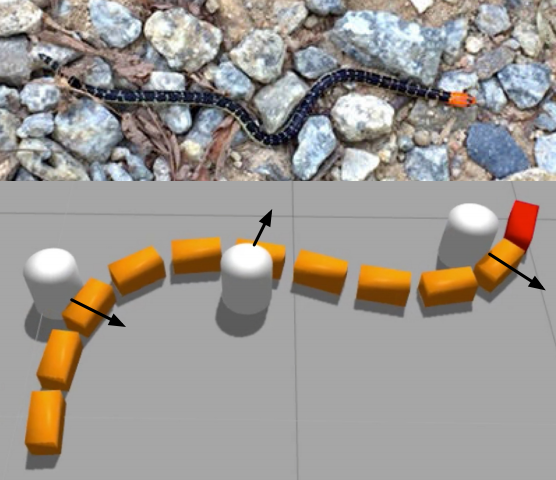
\includegraphics[width=0.6\textwidth]{figures/theory/oal.PNG}
    \caption{Obstacle-aided locomotion illustration \cite{sanfilippo2017snakesim}}
    \label{fig:oal}
\end{figure}